\subsubsection{Iluminação de interiores}\label {section: iluminacao_interiores}
	\begin{enumerate}
		\item Para a correta localização das fontes luminosas, a contratada, sempre que possível disporá as luminárias de forma simétrica a fim de garantir um bom bom fator de uniformidade (vide exemplo na figura \ref*{fig: disposicao}). Quaisquer disposições em contrário, a fiscalização deverá ser consultada.
		\begin{figure}[H]
			\centering
			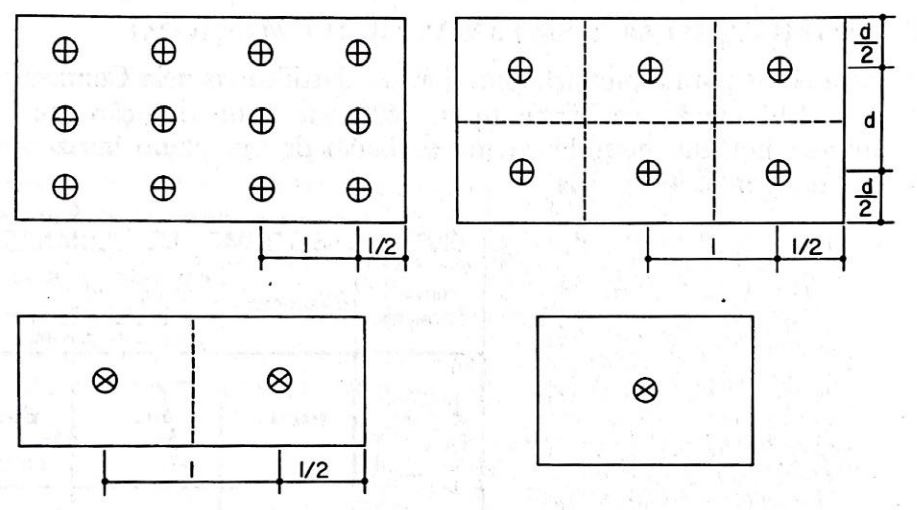
\includegraphics[width=\textwidth]{Figures/3. Lighting/light-disposicao.jpg}
			\hfill
			\caption{Disposição típicas de montagem para luminárias de iluminação de interior}  Referência \cite{de1987iluminação} p.112
			\label{fig: disposicao}
		\end{figure}
		
		\item Em instalações embutidas deverá ser utilizada a linha "PIALPLUS" da Legrand como referência técnica para interruptores e tampas
		
		\item Em instalações aparentes deverá ser utilizada a linha "Condulete TOP" da Tigre ou as linhas disponíveis da Wetzel como referência técnica para interruptores e tampas montados em conduletes de PVC
		
		\item Em instalações aparentes deverá ser utilizada as linhas disponíveis da Wetzel como referência técnica para interruptores e tampas montados em conduletes de alumínio
		
		\item\label{light:wc1}Em circuito de iluminação de banheiros e lavábulos será permitido conectar tomadas de uso geral (até 2 tomadas de 200W) ao referido circuito.
		
		\item\label{light:wc2}Em circuito de iluminação de banheiros e lavábulos será permitido conectar renovadores de ar do tipo "ventokit".
		
		\item Tomadas de uso geral não podem ser conectadas a circuitos de iluminação, a exceção das preconizadas nos itens \ref*{light:wc1} e \ref*{light:wc2}
		
		\item Em biotérios a contratada deverá prever um sistema de iluminação totalmente dimerizável
		
		\item Em Laboratórios NB3 ou NBA3 as luminárias dimensionadas serão do tipo herméricas
		\begin{enumerate}
			\item Laboratórios NB3 ou NBA3 com pavimento técnico a contratada deverá prever a remoção ou substituição dos equipamentos pelo referido pavimento, indicando em detalhe de projeto e notas
			\item Laboratórios NB3 ou NBA3 sem pavimento técnico e com forro de gesso, a contratada deverá prever em projeto que a face que possui o difusor da luminária irá facear o gesso e garantir a estanqueidade da área por sobre o gesso quando for necessário efetuar a manutenção da mesma.
			\item Demais casos deverão ser analisados pela contratada e discutidos com a Engenharia da COGIC.
		\end{enumerate}

		\item\label{light:encaixe10A}Nos caso dos encaixes rápidos utilizarem o conjunto tomada/plugue, deverá ser utilizada uma tomada de 10A
		
		\item As luminárias deverão ser projetadas tendo-se em mente a utilização de engate-rápido através de plugues e tomadas, ou dispositivos equivalentes, devendo a mesma ser indicada em nota e detalhada em projeto. Dois exemplos a seguir.
		
		\begin{figure}[H]
			\centering
			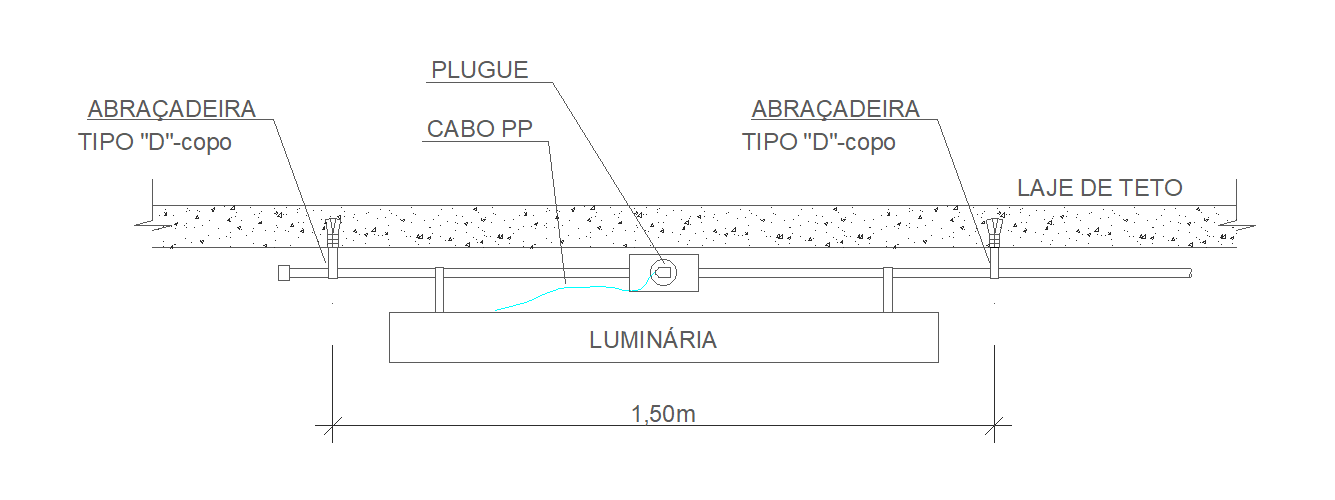
\includegraphics[width=\textwidth]{Figures/3. Lighting/light-engate rapido1.png}
			\hfill
			\caption{Encaixe rápido usando condulete e plugue de tomada ex.1}
			\label{fig: engate-rapido1}
		\end{figure}
		\begin{figure}[H]
			\centering
			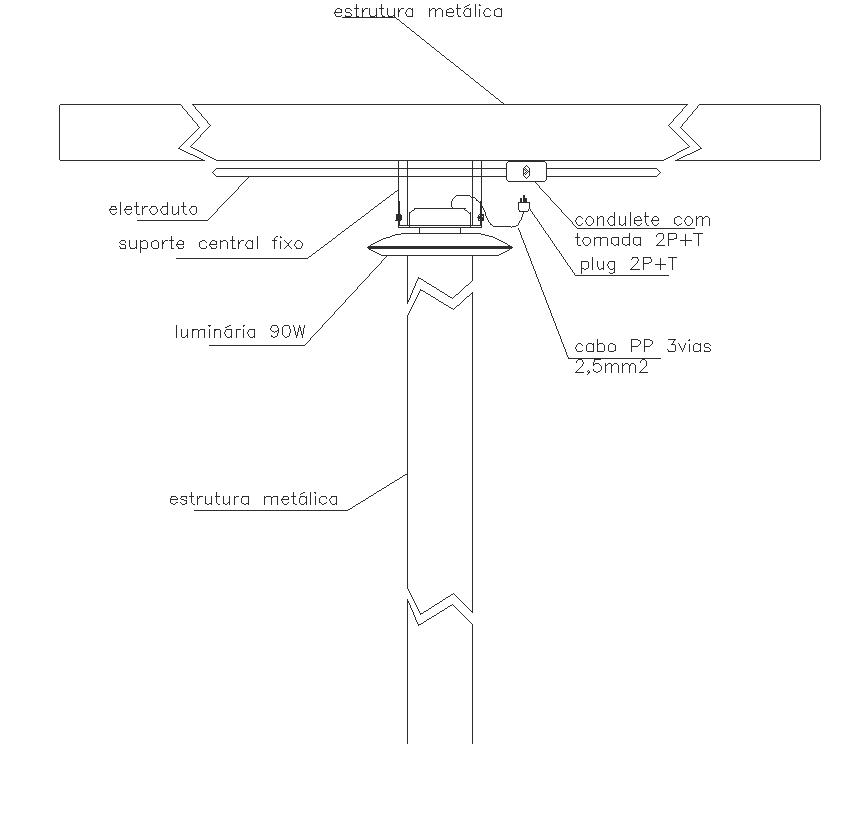
\includegraphics[scale=0.25]{Figures/3. Lighting/light-engate rapido2.png}
			\hfill
			\caption{Encaixe rápido usando condulete e plugue de tomada ex. 2}
			\label{fig: engate-rapido2}
		\end{figure}


		\item Luminárias instaladas em corredores deverão ser instaladas no sentido longitudinal a fim de obter um melhor rendimento no brilho e evitar ofuscamento. Melhores referências e explicações pode ser obtidas em \cite{simons2008lighting} p.74-75 e \cite{van2019interior} p.413.
		
		\item Luminárias em corredores só poderão ser instaladas no sentido transversal caso alguma exceção impossibilite a montagem no sentido longitudinal
	
	\end{enumerate}